%\documentclass[a4paper, 11pt]{article}

% HFUT_Courge_Project
% Typeset XeLatex
\documentclass[UTF8]{ctexart}
\usepackage{fancyhdr}
\usepackage{graphicx}
\usepackage{titlesec}
\usepackage{titletoc}
\usepackage{listings}
\usepackage{appendix}
\usepackage{bm, amsmath,amsfonts}
\usepackage{multirow}
\usepackage[a4paper,left=3.4cm,right=3cm,top=1.65cm,bottom=2.54cm]{geometry}
\usepackage{algorithm, algorithmic}
\renewcommand{\contentsname}{\zihao{3} 目\quad 录}
\renewcommand{\abstractname}{\zihao{3} 摘\quad 要}
%页眉页脚设置
\pagestyle{fancy}
\fancyhf{}
\cfoot{\thepage}
\rhead{\kaishu~生物智能与算法课程报告~}

%代码设置
\RequirePackage{listings}
\RequirePackage{xcolor}
\definecolor{dkgreen}{rgb}{0,0.6,0}
\definecolor{gray}{rgb}{0.5,0.5,0.5}
\definecolor{mauve}{rgb}{0.58,0,0.82}
\lstset{
numbers=left,  
frame=tb,
aboveskip=3mm,
belowskip=3mm,
showstringspaces=false,
columns=flexible,
framerule=1pt,
rulecolor=\color{gray!35},
backgroundcolor=\color{gray!5},
basicstyle={\ttfamily},
numberstyle=\tiny\color{gray},
keywordstyle=\color{blue},
commentstyle=\color{dkgreen},
stringstyle=\color{mauve},
breaklines=true,
breakatwhitespace=true,
tabsize=3,
}
%正文部分
\begin{document}
\begin{titlepage}
\centering
\vspace*{1.75cm}
\quad
\includegraphics[width=15cm,height=4cm]{zju.png}\\
\vspace*{1cm}
{\fontsize{40pt}\baselineskip 生\ 物\ 智\ 能\ 与\ 算\ 法\vskip 0.5cm 课\ 程\ 报\ 告}
 \vskip 5cm
 \fontsize{19pt}\baselineskip
 \makebox[30mm]{题\qquad\qquad 目}
 \underline{\makebox[75mm][c]{猫群算法}}\\%在这里修改成自己的题目
 \vskip 1.0cm
 \makebox[30mm]{学生姓名}
 \underline{\makebox[75mm][c]{ 方学成}}\\
 \vskip 1.0cm
 \makebox[30mm]{学\qquad\qquad 号}
 \underline{\makebox[75mm][c]{ \LARGE 21721228}}\\
 \vskip 1.0cm
 \makebox[30mm]{学\qquad\qquad 院}
 \underline{\makebox[75mm][c]{ 计算机科学与技术}}\\
 \vskip 1.2cm
 \LARGE \textbf{2018}~年~\textbf{4}~月~\textbf{30}~日		 
\end{titlepage}

 \begin{abstract}
 	\pagestyle{plain}
 	\thispagestyle{empty}
 	\zihao{-4}
\par 猫群算法作为一种群智能优化算法,有较快的收敛速度、向他人学习等优点,但国内目前对它的研究还处在起步阶段,所以做这方面的尝试性研究。通过引入交换子概念和改进猫的行为模式将算法用于求解TSP。最后通过仿真,并将实验结果与已知最优解相比较,验证了该算法的有效性。这不仅拓宽了猫群算法的应用范围,也给求解TSP等路径优化问题提供一种新的解决办法。
\\[0.5cm]
\textbf{关键字}:\quad 猫群算法 \quad 路径优化 \quad TSP
\newpage
\end{abstract}

\tableofcontents%%目录生成


\newpage
\setcounter{page}{1}
\begin{section}
{算法背景}\indent 提出背景:群智能优化算法是一种比较热门的计算技术,已成为系统优化、信息科学等相关领域中越来越重视的一部分。其中研究相对成熟的智能算法有遗传算法、粒子群算法、蚁群算法等。群智能算法在大规模优化问题如图像处理、模式识别等有着明显的计算速度快、收敛性能好等优势。\\ \indent 猫群算法(CSO)是2006年由台湾学者Chu等人通过观察猫群在日常生活中的行为提出来的一种新型群体智能算法。猫群算法与遗传算法类似,是基于迭代的优化方法,但是没有遗传算法的交叉算子,易实现,且拥有全局搜索、较快收敛速度等优点。\\ \indent TSP是一个经典的NP完全问题,目前已提出多种改进的群智能算法用于求解TSP,而且取得了比较好的效果。相比于粒子群算法、遗传算法等群智能算法,猫群算法的猫有其独特的跟踪、搜寻两种模式,使其兼顾了较好的全局搜索性质和不易陷入局部最优解两种优势,而且跟踪模式下的猫所处的模式类似粒子群算法中粒子的社会模式,能在处理TSP这种拥有较大解规模的问题里拥有较快的收敛速度。
\end{section}
\begin{section}
{猫群算法概述}\indent 猫群算法是研究人员通过观察自然界猫群的生活习性提出来的一种智能算法。该算法把猫群分成跟踪和搜寻两种模式。每只猫即对应问题的一个解。每只猫的属性由猫的速度、猫的适应值、猫处于跟踪或搜寻模式的标志值(通常为0或1)组成。每只猫处于初始位置,然后通过每只猫的标志值判断猫处于搜寻还是跟踪模式。若猫处于跟踪模式,则执行跟踪算子;若猫处于搜寻模式,则执行搜寻算子。最后使得猫处于一个新的位置,并保留最优猫直至算法满足结束条件。\\ \indent猫群算法的基本流程分为以下五步:\\

\begin{itemize}
	\item{初始化猫群。}
	\item{根据分组率将猫群随机划分为跟踪和搜寻两种模式。}
	\item{根据猫的标志值对猫执行相应的算子进行位置更新。}
	\item{计算每只猫的适应度,记录并保留适应度最优的猫。}
	\item{若满足结束条件则终止算法,否则再返回第二步。}
\end{itemize}
\indent 猫群算法的基本流程如图1所示。
\begin{figure}[htbp]
	\centering
	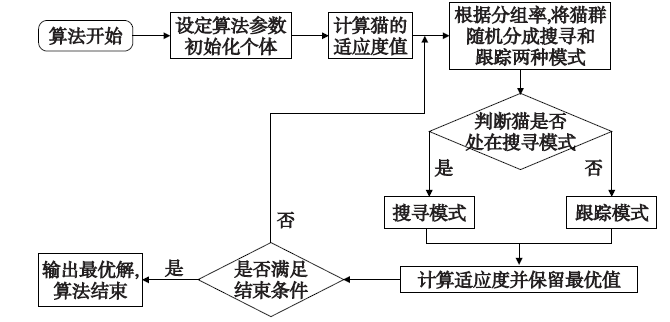
\includegraphics[width=0.8\textwidth]{pic/cat1.png}
	\caption{猫群算法的基本流程}
\end{figure}
\end{section}
\indent 主要参数介绍如下:\\
\begin{itemize}
	\item{猫群规模N,即猫的初始数量,由具体问题来确定。较大的猫群可以扩大搜索空间,但也增加了算法的复杂度,较小的猫群能较快收敛,但也容易陷入局部最优。}
	\item{分组率mr。将猫群随机分成两组,模拟现实生活中大部分猫处在搜寻状态,少量的猫处于跟踪模式,通常该参数取一个较小的值。}
	\item{个体猫上每个基因的改变范围srd。类似于遗传算法的变异概率,进行基因改变是为了增加解的多样性防止算法陷入局部最优。改变范围太小则不容易产生新解,范围太大则容易使算法变成随机搜索。}
	\item{最大迭代次数maxiter。由实验的具体问题而定,若迭代次数过大,可能算法已经收敛,会增加不必要的运算时间,若迭代次数过小,则容易出现早熟现象。}
\end{itemize}
\begin{subsection}
{跟踪模式描述}跟踪模式是模拟猫处于跟踪状态下建立的模型。在该模式下,通过改变猫的每一维速度来改变猫的位置。跟踪模式可以通过以下两步来描述:\\a) 速度的更新。\\ \indent整个猫群经历过的最好位置, 即目前搜索到的最优解,记做 $X_{best}$ 。每只猫的速度记做$v_i ={v_{i1},v_{i2},...,v_{id}}$,每只猫根据公式(1) 来更新自己的速度。$$v_{i,d}(t+1) = v^{i,d}(t) + r^* c^*(X_{best,d}(t) - x_{i,d}(t)),d = 1,2,...,M (1) $$ 
$v_{i,d}(t+1)$表示更新后第 i 只猫在第 d 维的速度值,M 为维数大小; 
$X_{best,d}(t)$ 表示猫群中当前具有最好适应度值的猫的位置; 
$x_{i,d}(t)$ 指当前第 i 只 猫在第 d 维的位置,\\c 是个常量,其值需要根据不同的问题而定。
r 是一个[0,1]之间的随机值。\\b) 位置的更新。\\ \indent 每只猫根据式(2)更新自己的位置。$$X_k^d(t+1) = X_k^d(t) + V_k^d(t+1),    (2)$$\\其中:$X_k^d(t+1)$表示第k只猫更新位置后的第d维分量。\\ \indent 猫群算法的跟踪模式流程如图2所示。
\end{subsection}

\begin{subsection}
{搜寻模式描述}搜寻模式是模拟猫在四处搜索并寻找下一个地点所建立的模型。在该状态下,定义了记忆池为每一只猫的搜寻记忆大小,每只猫根据适应度的大小从记忆池中选择一个最好的位置。搜寻模式的工作分为以下三步:\\
\begin{itemize}
	\item{复制自身位置。每只猫将自身位置在记忆池中复制K份,记忆池的大小为K。}
	\item{执行变异算子。对记忆池中的每只猫执行变异算子,使每只猫达到新的位置。每只猫的解基因需要改变的个数和每一个基因改变的范围是算法开始设定的。}
	\item{计算记忆池中每只猫的适应度,并将池中适应度最高的猫代替当前猫,完成位置更新。}
\end{itemize}
\indent 猫群算法的搜寻模式流程如图3所示。
\begin{figure}[htbp]
	\centering
	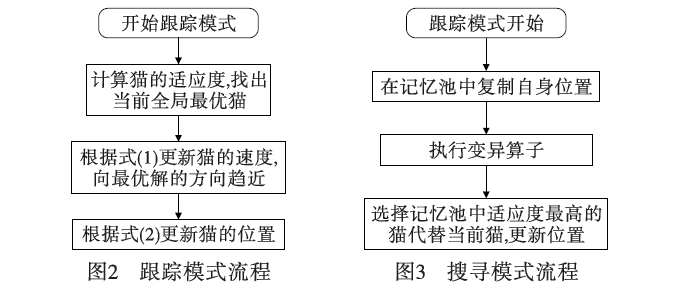
\includegraphics[width=0.8\textwidth]{pic/cat2.png}
\end{figure}
\end{subsection}
\begin{section}
{算法简述}
\end{section}
\begin{subsection}
{TSP的数学模型}TSP即旅行商问题,是一个经典的NP难题,指的是一名旅行商要经过多个城市,在经过每个城市一次且一次后再回到出
发城市的最短距离。如何确定最短距离,用数学语言描述就是在n个点的赋权图中找一条距离最短的哈密尔顿圈。
\\ \indent 设$d_ij$为城市i与j之间的距离,则目标函数为城市哈密尔顿圈总长度。
\\ \indent 随着城市的数目增加,其算法复杂性呈指数增加,会出现所谓的组合爆炸现象。它的解是多维的、多局部极值的、趋于
无穷大的。所以当城市数目过大时,用枚举搜索策略几乎是不可能做到的。
\end{subsection}
\begin{subsection}
{改进的猫群算法} 在本文中,各个术语的代表如下:
\\ \indent 猫:算法中的一个解,对应TSP中的一个路径解。
\\ \indent 猫群:TSP中所有的路径解。
\\ \indent 适应度:猫所处位置的适应度,在算法中表现为猫所处位置的优劣,在TSP中代表路径解的长度。
\\ \indent 记忆池:在搜寻模式下,记忆池的大小代表猫能够搜索的地点数量,通过变异算子改变原值,使记忆池储存了猫自身邻域内能够搜索的新地点。猫将依据适应度的大小从记忆池中选择一个最好的位置点。
\\ \indent 个体上每个基因的改变范围:在算法开始之前设定,在本文中代表路径解每一维的变异概率。
\\ \indent 每个个体上需要改变的基因个数:在算法开始设定,在本文中代表路径解可变异的维数。
\\ \indent 分组率:分组率将猫群随机分为跟踪模式和搜寻模式两组,指的是跟踪模式的猫在猫群中所占的比例,通常为较小的数。
\\ \indent 对猫群算法的改进就是在跟踪模式中引入交换子和交换序的概念,对基本猫群算法重新定义,将其应用于求解TSP中。
\\ \indent CSO跟踪算子定义如下:
\\ \indent 猫的位置,即为解,在本文算法中,猫的位置$X = {X_1,X_2,...,X_n}$,$X_n$为城市点,n为城市的个数,代表城市遍历的顺序为$X = {X_1,X_2,...,X_n}$。
\\ \indent 设城市序列A = $X = {X_1,X_2,...,X_n}$定义交换子S=(j,k)作用为交换解中$X_j$和$X_k$的位置。对解序列A用交换子(j,k)进行交换可得新解$X = {X_1,X_2,...X_j,...X_k,...X_n}$,$X_n$定义位置与交换子的加法为交换子作用在原解序列上得到的新解序列即B = A+S。如A=(1,3,2,4,5),B=(3,1,2,4,5),则可用交换子S = (2,1)对解序列A里的点进行交换得到解序列B,即(1,3,2,4,5)+(2,1)=(3,1,2,4,5),同理定义位置与位置之间的减法为一个解到另一个解所需做的交换即B-A=S,如(3,1,2,4,5)-(1,3,2,4,5)=(2,1)。
\\ \indent 由一个或多个交换子组成的有序队列为交换序。如A=(1,3,2,4,5),B=(3,1,4,5,2),则可用三个交换子(1,2),(3,5),(4,5)依次对A中的点进行交换得到B,SS={(1,2),(3,5),(4,5)}为交换序。定义位置与交换序的加法为交换序里的交换子依次作用在原解上得到的新解即B=A+SS。
\\ \indent 猫的速度。猫的速度为交换序,速度$V = {V_1,V_2,...,V_n}$,$V_N$为交换子。
\\ \indent速度的数乘。速度的数乘有概率意义,$V_A = {C·V_b}$,其中c∈[0,1]是一个常数,在计算$V_a$时,对$V_b$中每一维速度生成一个(0,1)的随机数。
\\ \indent基本的猫群算法分组率是个固定值,在每次更新猫的位置时都会分配固定数量的猫在两个模式下,但是这样猫群算法的搜索能力不能有效地提高。针对此问题本文引用了分组率随时间变化的猫行为模式,即$$mr = mr_max - (mr_max - mr_min)·iter/maxiter$$其中iter为当前迭代数。此方法可以在算法的前期用比例较多的跟踪猫提高全局搜索能力,从而提高算法收敛的速度;后期则用比例较多的搜寻猫来使算法更好地跳出局部最优解。
\\ \indent在搜寻模式里引入类似遗传算法的变异算子,在搜寻模式下路径解的城市序列根据概率srd进行变异,如(1,3,2,5,4)变为(1,2,3,5,4),设置基因改变的个数即城市点变异的个数的范围smp。
\\ \indent算法流程如下:
\begin{itemize}
	\item{参数初始化;}
	\item{初始化猫群,随机产生N个初始解;}
	\item{计算每只猫的适应度,适应度函数为$F = \sum x_{ij}d_{ij}$;}
	\item{所有的猫按分组率随机分配到搜寻模式组和跟踪模式组;}
	\item{判断每只猫所处的模式并对两组内的猫个体执行相应的模式算子,计算每只猫的适应度,更新全局最优猫;}
	\item{当更新完所有猫后,若未到达最大迭代次数,转至第四步重新计算,直至满足最大迭代数maxiter,则结束进化进程;}
	\item{找出最优路径并做2—opt,如果更优,则改进,否则保持原最优路径。}
\end{itemize}
\end{subsection}
\begin{section}
{结论与分析}在参数初始化中,选取中国31省会路径问题为例,猫群规模N=100,最大迭代次数maxiter=100,常数c=0.5,记忆池K=5,城市点变异概率srd=0.2,城市点变异个数$smp_max$=3,$smp_max$=1。图4为分组率mr分别取0.4和随时间变化取$mr_max$=0.6和$mr_min=0.3$两种模式下的猫群算法运行10次后的结果。
\\ \indent从图中可以看出,猫群算法对该问题的解均是收敛的,引入分组率取随时间变化策略的CSO的收敛速度要快于分组率取定值的CSO,而且总体来说改进后的CSO算法效果要较好。
\\ \indent图5为改进后猫群算法运行10次后取得的最优值已经处在最优解的范围里。
\begin{figure}[htbp]
	\centering
	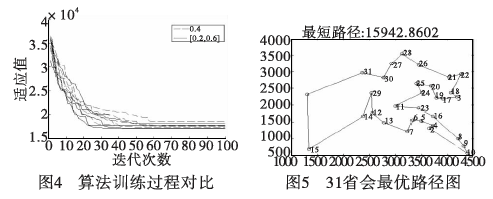
\includegraphics[width=0.8\textwidth]{pic/cat4.png}
\end{figure}
\end{section}
\begin{section}
{总结}将猫群算法与粒子群算法和蚁群算法为代表的经典算法相比较时,在部分已知例子上的最优解相差并不大。本文算法与果蝇算法和湖水能量优化算法为代表的新型智能算法相比较时,在部分已知例子上的最优解要略优于新型智能算法,且在TSP规模较小时,猫群算法所得的解总能收敛在最优解的范围中,当TSP规模比较大时,猫群算法也能取得较好的结果,并且解也总是收敛的,可以证明猫群算法应
用在TSP上的有效性。猫群算法是新型群智能算法,发展还不成熟,接下来对猫群算法的研究还有很多路要走。
\\ \indent
\end{section}
\newpage
\begin{thebibliography}{123} 
\bibitem{fish_bib1} 杨进, 郑允, 马良. 改进的猫群算法求解TSP[J]. 计算机应用研究, 2017(12):3607-3610.
\bibitem{fish_bib2} 黄岚,王康平,周春光,等.粒子群优化算法求解旅行商问题[J].吉林大学学报:理学版,2003,41(4):477-480.
\bibitem{fish_bib3}王光彪,杨淑莹,冯帆,等.基于猫群算法的图像分类研究[J].天津理工大学学报,2011,27(21):35-39.
\end{thebibliography}
%\newpage
%\begin{appendices}
%\section{程序代码}
%\begin{lstlisting}[language=C++,escapeinside=``]
%#include<iostream>
%using namespace std;
%int main
%{
%cout<<"Hello world!"<<endl;//`输出`
%return 0;
%}
%\end{lstlisting}
%\end{appendices}

\end{document}












